\def\mytitle{IOT ASSIGNMENT}
\def\myauthor{R.Radhika}
\def\contact{r170234@rguktrkv.ac.in}
\def\mymodule{Future Wireless Communications (FWC)}
\documentclass[10pt, a4paper]{article}
\usepackage[a4paper,outer=1.5cm,inner=1.5cm,top=1.75cm,bottom=1.5cm]{geometry}
\twocolumn
\usepackage{graphicx}
\graphicspath{{./images/}}
\usepackage[colorlinks,linkcolor={black},citecolor={blue!80!black},urlcolor={blue!80!black}]{hyperref}
\usepackage[parfill]{parskip}
\usepackage{lmodern}
\usepackage{tikz}

\usepackage{karnaugh-map}

\usepackage{tabularx}
%\documentclass{article}
%\documentclass[tikz, border=2mm]{standalone}
%\usepackage{tikz}
\usepackage{circuitikz}
\usetikzlibrary{calc}

\renewcommand*\familydefault{\sfdefault}
\usepackage{watermark}
\usepackage{lipsum}
\usepackage{xcolor}
\usepackage{listings}
\usepackage{float}
\usepackage{titlesec}

\titlespacing{\subsection}{1pt}{\parskip}{3pt}
\titlespacing{\subsubsection}{0pt}{\parskip}{-\parskip}
\titlespacing{\paragraph}{0pt}{\parskip}{\parskip}
\newcommand{\figuremacro}[5]{
    \begin{figure}[#1]
        \centering
        \includegraphics[width=#5\columnwidth]{#2}
        \caption[#3]{\textbf{#3}#4}
        \label{fig:#2}
    \end{figure}
}

\lstset{
frame=single, 
breaklines=true,
columns=fullflexible
}

%\thiswatermark{\centering \put(400,-128.0){\includegraphics[scale=0.3]{logo}} }
\title{\mytitle}
\author{\myauthor\hspace{1em}\\\contact\\IITH\hspace{0.5em}-\hspace{0.6em}\mymodule}
\date{19-09-2022}
\begin{document}
  \maketitle
  \tableofcontents
  \begin{abstract}
      This manual shows that move the content of one register to another register  :
%\figuremacro{h}{diag}{}{}{0.9}
  \end{abstract}

  
\section{Introduction}
    \subsection{7474 IC:}
This IC contains 2 D-flip flops.\\
For this section total of 4 flip-flops(2 ICs) are required since we need to design a 4-bit shift register.

\subsection{Arduino:}
    In Arduino Uno we generate the clock pulse which is given to the each and every flip-flop by default.\\
    We take 5 volts and Ground as the supply to the bread board from the Arduino board.


  \section{Components}
  \begin{tabularx}{0.4\textwidth} { 
  | >{\centering\arraybackslash}X 
  | >{\centering\arraybackslash}X 
  | >{\centering\arraybackslash}X
  | >{\centering\arraybackslash}X | }
\hline
 \textbf{Component}& \textbf{Values} & \textbf{Quantity}\\
\hline
Arduino & UNO & 1 \\  
\hline
JumperWires& M-M & 20 \\ 
\hline
Breadboard &  & 1 \\
\hline
IC & 7447 &2 \\
\hline
\end{tabularx}

\section{PIN Diagram}
\begin{center}
   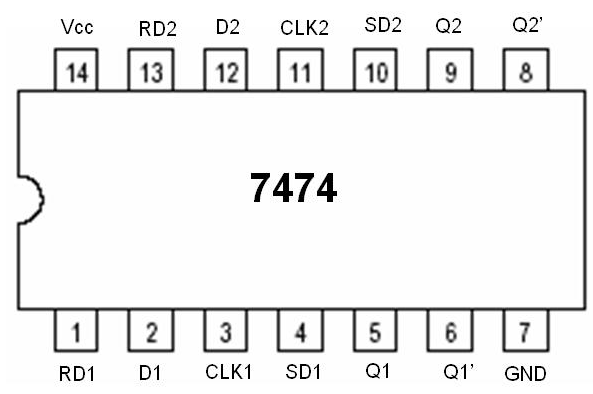
\includegraphics[width=3in]{pindiagram.png}
\end{center}


\begin{center}
Figure.a
\end{center}

\section{Truth Table}
  \begin{tabularx}{0.46\textwidth} { 
  | >{\centering\arraybackslash}X 
  | >{\centering\arraybackslash}X 
  | >{\centering\arraybackslash}X
  | >{\centering\arraybackslash}X 
  | >{\centering\arraybackslash}X 
  | >{\centering\arraybackslash}X 
  | >{\centering\arraybackslash}X 
  | >{\centering\arraybackslash}X 
  | >{\centering\arraybackslash}X 
  | >{\centering\arraybackslash}X | }


\hline
D1 & Q1=D2 & Q2=D3 & Q3=D4  & Q4\\
\hline
0 & 0 & 0 & 0 & 0 \\  
\hline
1 & 1 & 0 & 0 & 0 \\ 
\hline
1 & 1 & 1 & 0 & 0 \\
\hline
0 & 0 & 1 & 1 & 0 \\
\hline
0 & 0 & 0 & 1 & 1 \\  
\hline
0 & 0 & 0 & 0 & 1\\ 
\hline
0 & 0 & 0 & 0 & 0 \\
\hline
\end{tabularx}
\begin{center}
 Truth table for 0110
\end{center}

\section{Circuit Diagram}
\begin{figure}
\centering
    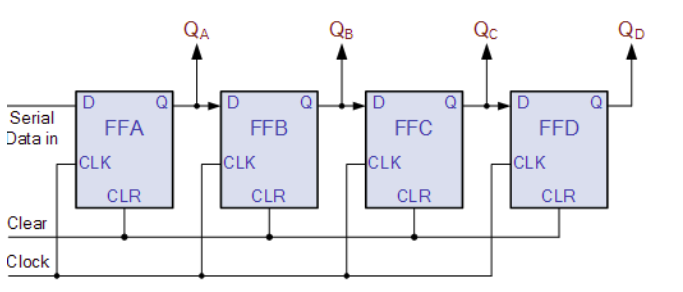
\includegraphics[width=4in]{SIPOregister.png}
\end{figure}
\begin{center}
Figure.b
 \end{center}
    \paragraph{4-bit shift register:}
 1.It has 4 D-flip flops.\\
 2.Verify the output for the sequence by changing the D1 pin to Vcc and Ground for different clock cycles.\\
 3.It has 4 outputs i.e Q1, Q2, Q3 and Q4.\\
 4. We need to give the input from MSB to LSB.\\
        
    \paragraph{Problem-1}
    1. Connect the circuit as per the above diagram.\\
    2. Execute the circuit using the below code.\\
	\paragraph{Problem-2}
1. Same circuit can be implemented by without IC display to the Q1, Q2, Q3 AND Q4 respectively.\\
2. Execute the circuit using the below code.\\
\section{ Circuit Implementation}
  \begin{tabularx}{0.86\textwidth} { 
  | >{\centering\arraybackslash}X 
  | >{\centering\arraybackslash}X 
  | >{\centering\arraybackslash}X
  | >{\centering\arraybackslash}X 
  | >{\centering\arraybackslash}X 
  | >{\centering\arraybackslash}X 
  | >{\centering\arraybackslash}X 
  | >{\centering\arraybackslash}X 
  | >{\centering\arraybackslash}X
  | >{\centering\arraybackslash}X
  | >{\centering\arraybackslash}X
  | >{\centering\arraybackslash}X
  | >{\centering\arraybackslash}X
  | >{\centering\arraybackslash}X
  | >{\centering\arraybackslash}X 
  | >{\centering\arraybackslash}X | }


\hline
\textbf{Ard} & \textbf{D13} & \textbf{D13} &  &  &  & \textbf{Vcc} & \textbf{Vcc} & \textbf{Vcc} & \textbf{Vcc} & \textbf{Vcc} & \textbf{Gnd} &  &  &  & \\  
\hline
\textbf{7474} & 3 & 11 & 5-12 & 9 &  & 1 & 4 & 10 & 13 & 14 & 7 & 5 & 9 &  &  \\
\hline
\textbf{7474} & 3 & 11 &  & 2 & 5-12 & 1 & 4 & 10 & 13 & 14 & 7 &  &  & 5 & 9  \\
\hline
\textbf{LED} &  &  &  &  &  &  &  &  &  &  &  & led1 & led2 & led3 & led4  \\
\hline
\end{tabularx}

\begin{center}
    Connections
\end{center}
        
        \bibliographystyle{ieeetr}
 \subsection{The steps for implementation:}
  Flash the following setup code through USB-UART using laptop
\begin{lstlisting}
svn co https://github.com/Radhikarkv/fwcproject.git/trunk/iot/codes/setup
cd  setup
pio run
pio run -t upload
\end{lstlisting}
after entering your wifi username and password (in quotes below)
\begin{lstlisting}
#define STASSID "..." // Add your network credentials
#define STAPSK  "..."
\end{lstlisting}
in src/main.cpp file
 You can notice that vaman will be connnected to the network credentials provided above.Connect your laptop to the same network ,You should be able to find the ip address of your vaman-esp on laptop using 
\begin{lstlisting}
ifconfig
nmap -sn 192.168.6.1/24
\end{lstlisting}
where your computer's ip address is the output of ifconfig and given by 192.168.6.x
Login to termux-ubuntu on the android device and execute the following commands:
\begin{lstlisting}
proot-distro login debian
cd  /data/data/com.termux/files/home/
mkdir iot
svn co https://github.com/Radhikarkv/fwcproject.git/trunk/iot/codes/ota
cd codes
\end{lstlisting}
\begin{center}
\fbox{\parbox{8cm}{\url{https://github.com/Radhikarkv/fwcproject.git/blob/main/iot/codes/ota/src/main.cpp}}}
\end{center}
through 
\begin{lstlisting}
pio run 
pio run -t nobuild -t upload --upload-port ip_addres_of_esp
\end{lstlisting}
where you may replace the above ip address with the ip address of your vaman-esp.
\end{document}
